%!TEX encoding = utf-8
\documentclass[12pt]{article}
\usepackage{amsmath}
\usepackage{amssymb}
\usepackage{amsfonts}
\usepackage{amsthm}
\usepackage{mathrsfs}
\usepackage{mathtools}
\usepackage{kotex}
\usepackage{tikz}
\usepackage{geometry}
\geometry{
    top = 20mm,
    left = 20mm,
    right = 20mm,
    bottom = 20mm
}

\begin{document}

\begin{center}
    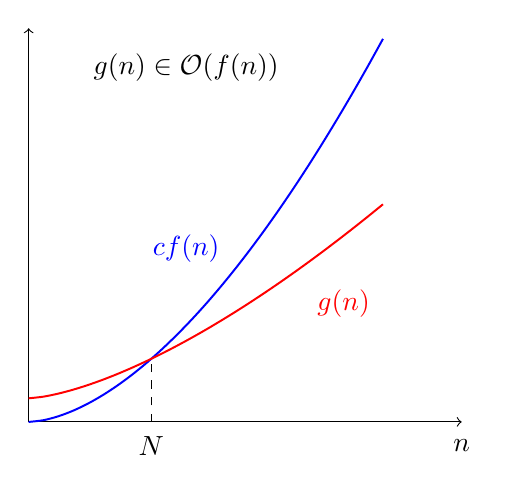
\begin{tikzpicture}
        \draw[->] (0, 0) -- (5.5, 0);
        \draw[->] (0, 0) -- (0, 5);
        \draw[line width=0.25mm, scale=0.15, domain=0:30, smooth, variable=\x, blue] plot ({\x}, {0.1 * \x^1.7});
        \draw[line width=0.25mm, scale=0.15, domain=0:30, smooth, variable=\x, red] plot ({\x}, {0.1 * \x^1.5 + 2});
        \draw[dashed] (1.5585, 0) -- (1.5585, 0.8024);
        \draw (1.5585, -0.3) node {\(N\)};
        \draw (5.5, -0.3) node {\(n\)};
        \draw (2, 2.2) node {\color{blue} \(cf(n)\)};
        \draw (4, 1.5) node {\color{red} \(g(n)\)};
        \draw (2, 4.5) node {\(g(n) \in \mathcal{O}(f(n))\)};
    \end{tikzpicture}
\end{center}

\begin{center}
    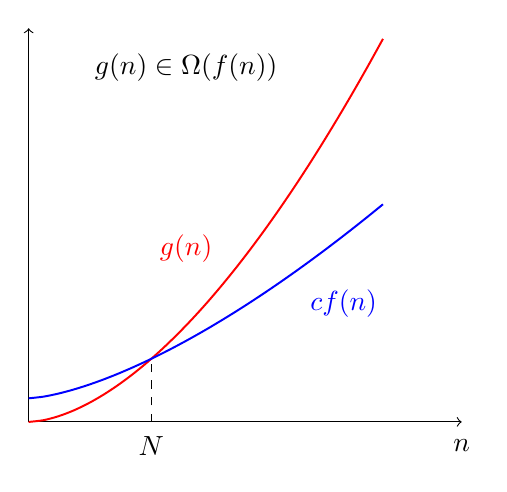
\begin{tikzpicture}
        \draw[->] (0, 0) -- (5.5, 0);
        \draw[->] (0, 0) -- (0, 5);
        \draw[line width=0.25mm, scale=0.15, domain=0:30, smooth, variable=\x, red] plot ({\x}, {0.1 * \x^1.7});
        \draw[line width=0.25mm, scale=0.15, domain=0:30, smooth, variable=\x, blue] plot ({\x}, {0.1 * \x^1.5 + 2});
        \draw[dashed] (1.5585, 0) -- (1.5585, 0.8024);
        \draw (1.5585, -0.3) node {\(N\)};
        \draw (5.5, -0.3) node {\(n\)};
        \draw (2, 2.2) node {\color{red} \(g(n)\)};
        \draw (4, 1.5) node {\color{blue} \(cf(n)\)};
        \draw (2, 4.5) node {\(g(n) \in \Omega(f(n))\)};
    \end{tikzpicture}
\end{center}

\begin{center}
    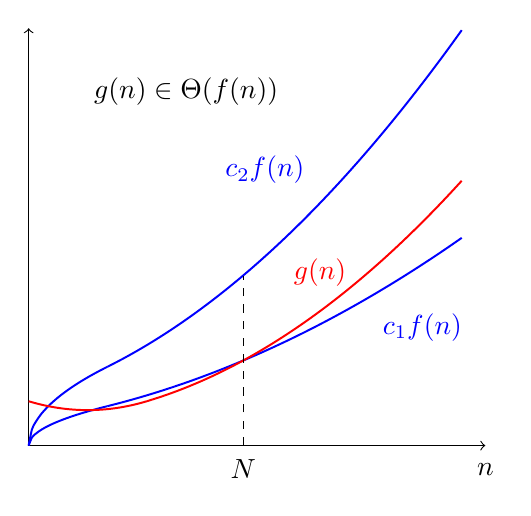
\begin{tikzpicture}
        \draw[->] (0, 0) -- (5.8, 0);
        \draw[->] (0, 0) -- (0, 5.3);
        \draw[line width=0.25mm, scale=1, domain=0:1, smooth, variable=\x, blue] plot ({\x}, {\x^0.5});
        \draw[line width=0.25mm, scale=1, domain=1:5.5, smooth, variable=\x, blue] plot ({\x}, {0.1 * \x^2 +0.3 * \x + 0.6});
        \draw[line width=0.25mm, scale=1, domain=0:1, smooth, variable=\x, blue] plot ({\x}, {0.5 * \x^0.5});
        \draw[line width=0.25mm, scale=1, domain=1:5.5, smooth, variable=\x, blue] plot ({\x}, {0.05 * \x^2 +0.15 * \x + 0.3});
        \draw[line width=0.25mm, scale=1, domain=0:1.5, smooth, variable=\x, red] plot ({\x}, {0.2 * (\x - 0.75)^2 + 0.45});
        \draw[line width=0.25mm, scale=1, domain=1.5:5.5, smooth, variable=\x, red] plot ({\x}, {0.1 * \x^2 + 0.3375});
        \draw[dashed] (2.7247, 0) -- (2.7247, 2.159);
        \draw (2.7247, -0.3) node {\(N\)};
        \draw (5.8, -0.3) node {\(n\)};
        \draw (3.7, 2.2) node {\color{red} \(g(n)\)};
        \draw (5, 1.5) node {\color{blue} \(c_1f(n)\)};
        \draw (3, 3.5) node {\color{blue} \(c_2f(n)\)};
        \draw (2, 4.5) node {\(g(n) \in \Theta	(f(n))\)};
    \end{tikzpicture}
\end{center}

\end{document}
